\subsection{Fitting}
    
    Luego de definirse un modelo para regresión, nos interesa encontrar el valor óptimo de $\beta$, es decir, de los parámetros desconocidos, tal que el error de la predicción es el mínimo posible. Para esto, primero definimos la ecuación que involucra a cada $Y_i$ con los $X_i$ y las $f_j$ en forma matricial, aprovechando que es una combinación lineal de funciones:
    
    \begin{equation}
\begin{bmatrix}
 Y_1 \\ \vdots \\ Y_{n} 
 \end{bmatrix}
 =
 \begin{pmatrix}
  f_1(X_{11}) && \ldots & f_k(X_{1k}) \\
  \vdots && \ddots & \vdots \\
  f_1(X_{n1}) && \ldots & f_k(X_{nk})
  \end{pmatrix}
  \times
  \begin{pmatrix}
  \beta_1 \\ \vdots \\ \beta_k
  \end{pmatrix}
  +
  \begin{pmatrix}
  e_1 \\ \vdots \\ e_k
  \end{pmatrix}
\end{equation}
    
    Luego, nos interesa minimizar cada $e_i$, que es equivalente a minimizar la norma del vector $e$. Luego, si dejamos el error en función de las demás variables, tenemos este sistema:
    
    \[ b - Ax = e  \implies ||b - Ax||_2 = ||e||_2 \]
    
    Donde b es el vector Y, A es la matriz anterior con elementos $f_i(X_{ji})$, $x$ es el vector $\beta$ a determinar, y $e$ es el vector de los errores individuales. Como queremos minimizar la norma de $e$, podemos plantear este sistema y obtendremos el x ($\beta$) que minimiza el $e$ (error):
    
    \[ \min_x  ||b - Ax||_2\]
    
    Transformando el problema de encontrar el $\beta$ óptimo a esto, podemos aplicar un método conocido para resolver esto.
    
    \subsubsection{CML (Cuadrados Mínimos Lineales)}
    
    Cuadrados mínimos lineales es un método utilizado para encontrar el $x$ que minimiza esa norma de manera directa. Para esto, utiliza lo que se llama \textit{Ecuaciones Normales} que transforma el problema en uno equivalente, basado en la resolución de un sistema lineal:
    
    \[ \min_x  ||b - Ax||_2 \iff A^T A x = A^T b\]
    
    Al método se le atribuye este nombre porque busca minimizar la norma, que termina siendo equivalente a minimizar la suma de cuadrados, que son las diferencias entre cada estimación y su valor real al cuadrado. Entonces, se obtiene un valor para el vector $x$, es decir nuestro $\beta$, que minimiza esta suma de cuadrados, que visto para el caso de regresión lineal gráficamente se ve así:
    
    \begin{figure}[H]
        \begin{center}
            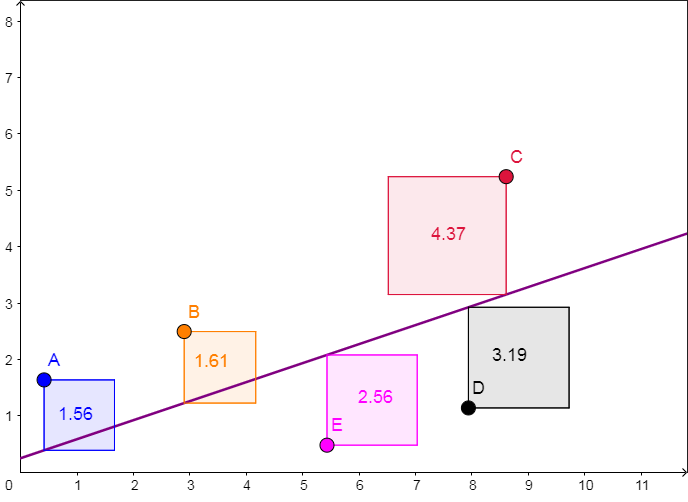
\includegraphics[scale=0.4]{img/explicaciones/CML-Line.png}
            \end{center}
    \end{figure}
    
    Donde la recta es la que minimiza las áreas de esos cuadrados, que surgen de hacer las diferencia entre lo que estimó la recta y el valor real, es decir, cada punto que aparece ahí.
   